%!TEX root = ../main.tex
\doublespacing
\chapter{Theoretical Background}
\label{chap:theory}
The following chapter describes the core concepts relevant to this thesis in more detail than Chapter \ref{chap:intro}. Here I discuss the various mechanisms for radio wave emission in the solar corona, with particular emphasis on the plasma emission process. I will also give an introduction to the mathematical formalisms of radio interferometry.
\section{Introductory Concepts in Plasma Physics}
Plasma was the name given by Langmuir to the new, exotic type of matter he was studying in the 1920s. It is essentially an ionized gas that exhibits quasi-neutrality on a macroscopic scale. Maxwell-Boltzman distributions.
\subsection{Plasma Frequency}
\section{Radio Emission Mechanisms in the Solar Corona}
\subsection{Bremstrahlung}
\subsection{Gyroemission}
\subsection{ECMI}
\subsection{Plasma Emission}
\section{Plasma Emission}
\label{sec:plasma}
In 1942 while Britain was on the look out for radar signals of enemy aircraft, a strong, noise like and highly variable signal was noticed by radar operators. Initially it was thought that Germany had managed to learn the secret of radar and create some sort of jamming device. On further investigation it was found that this jamming was in fact radio emission from the Sun. The discovery of this radio emission being associated with a major solar flare was kept secret until after the war and was published by \cite{Appleton1946}.
Since then a number of major advancements in both instrumentation and theory have occurred. A culmination of the theory of solar radio emission is laid out in the book by \cite{McLean1985} while worldwide, a number of extraordinary radio telescopes and interferometers such as the LOw Frequency ARray \cite[LOFAR,][]{VanHaarlem2013}, the Nan\c{c}ay Radio Heliograph and the Murchison Widefield Array (MWA), to name but a few, have been built.

Solar radio emission often comes in the form of bursts of varying timescales. These were initially classified into three types by \cite{Wild1950b} with a fourth and fifth type being discovered by \cite{Boischot1957} and \cite{Wild1959} respectively. Of these, the most frequently occurring are the so called Type III radio bursts. These are short bursts that can be observed over many frequencies and are found to be associated with solar flares \citep{Malville1962}. An initial study into how they are emitted was conducted by \cite{Ginzburg1958}.% This essay examines Type III bursts and in particular describes their observed characteristics, what causes them and the plasma emission process of their generation.

%\section{Process of Forming Type III Bursts} %(This is how they're made)}
For a Type III radio burst to be emitted, an electron must generate Langmuir waves in the plasma. These Langmuir waves then go on to generate electromagnetic transverse waves by coalescing with other waves or by decaying. Theses electromagnetic waves are the radio bursts that are observed. In this section the generation of Langmuir waves and the process of plasma emission are discussed.

\subsection{Generation of Langmuir Waves}
During magnetic reconnection in a solar flare electrons are accelerated along magnetic field lines. As these beams of electrons propagate, faster electrons begin to outpace slower electrons and stationary ions in the background plasma. This leads to a second peak on the Maxwell Boltzmann distribution of velocities as seen in Figure \ref{fig:Lwavegrowth}. Energy is transferred from electrons electrons travelling at the phase velocity, $v_{\phi}$ , to Langmuir waves creating a resonance.
The positive velocity gradient of this resonance means that there are more electrons with velocity greater than $v_{\phi}$ than there are electrons with velocities less than  $v_{\phi}$ (where energy is transferred from the wave to the particles), this causes Langmuir waves to become unstable and their magnitudes to grow exponentially. Particles with velocities near $v_{\phi}$ are in resonance with the Langmuir waves and drive this instability.

This instability is alleviated by what is known as quasi-linear relaxation \citep{Melrose1987} whereby the resonant behaviour of the electrons and Langmuir waves results in a plateau in the Maxwell Boltzmann distribution rather than a second peak. It can be shown that \citep{Vedenov1963} the electron distribution function, $f(v,t)$ where $\int f(v,t) dv = n_e$, and the spectral energy index of Langmuir waves, $W(v,t)$ such that $\int W(v,t) dv = E_L$ the total energy density, can be expressed as follows \citep{Reid2014},
\begin{equation}\label{eq:dfdt}
    \frac{\partial f(v,t)}{\partial t}=\frac{4 \pi^2 e^2}{m_e^2} \frac{\partial}{\partial v} \left( \frac{W}{v} \right) \frac{\partial f(v,t)}{\partial v}
\end{equation}

\begin{equation}\label{eq:dWdt}
    \frac{\partial W(v,t)}{\partial t}= \frac{\pi \omega_p}{n_e} v^2 W \frac{\partial f(v,t)}{\partial v}
\end{equation}

Equation \ref{eq:dWdt} shows that the growth rate of Langmuir waves is proportional to $\frac{\partial f(v,t)}{\partial v}$, hence a positive gradient in the Maxwell Boltzmann distribution leads to a growth in Langmuir waves. The right hand side of Eq. \ref{eq:dfdt} has a diffusion operator $D=\frac{W}{v}$. This states that the transfer of energy from particles to waves and back leads to the distribution function being smoothed out and eventually becoming a plateau. The evolution of $f(v,t)$ and $W(v,t)$ with time is shown in Figure \ref{fig:Lwavegrowth}. Figure \ref{fig:Lwavegrowth} shows how the plateau in the distribution function and a broadening in the spectral energy density develop as time progresses.

\begin{figure}
    \centering
    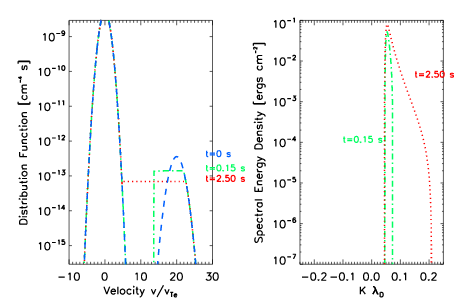
\includegraphics[width=0.75\columnwidth]{Images/L_wave_growth.png}
    \caption[Langmuir wave distriburtion function and spectral energy density.]{Left: Evolution of distribution function (normalised by the electron thermal velocity $v_{Te}=V_e$) in time. The diffusive term in \ref{eq:dfdt} causes the bump-on-tail Gaussian to turn into a plateau, thereby eliminating the instability caused by the positive velocity gradient. Right: The spectral energy density of generated Langmuir waves, x-axis normalised to the Debye length $\lambda_D=\sqrt{\frac{\epsilon_0 k_B T_e}{e^2 n_e}}$. As time passes the spectral range of Langmuir waves increases. Each panel shows successive times of t=0.15s (green, dot-dashed line) and t=2.50s (red, dotted line). \citep[Figure taken from][]{Reid2014}.} %(Figure taken from \citeauthor{Reid2014} \citeyear{Reid2014})}
    \label{fig:Lwavegrowth}
\end{figure}

\subsection{Wave-Wave Interaction}\label{Plasma Emission}
Wave-wave interaction concerns the processes by which three types of waves interact. These are: transverse (T) waves, Langmuir (L) waves and ion sound (S) waves, and have the following, respective dispersion relations,
$$ \omega=(\omega_p^2 +k^2c^2)^{\frac{1}{2}} $$
$$ \omega \cong \omega_p + \frac{3k^2V_e^2}{2 \omega_p}$$
$$ \omega = kv_s $$
where $V_e$ is the thermal velocity of electrons in the plasma, $v_s$ is the ion sound speed and $k$ is the wave vector. Only transverse waves with $\omega > \omega_p $ can escape and thus a plasma emission mechanism is a process that generates these transverse waves. 

As mentioned in Section \ref{characteristics}, Type III bursts have a harmonic structure associated with plasma emission at the plasma frequency and the second harmonic. Both of these transverse waves are formed in different three wave processes that will now be discussed.
In a plasma, due to scattering from other wave modes and ions in the plasma, a wave mode can be changed from one to the other. This is expressed in the equation 
$$ \sigma \rightleftarrows \sigma' + \sigma '' $$
where $\sigma$, $\sigma'$  and  $\sigma ''$ represent different wave modes. Conservation of energy and momentum state,
$$ \omega^{\sigma}(k)=\omega^{\sigma'}(k')+\omega^{\sigma''}(k'')$$
$$ k=k'+k''$$
where $ \omega^{\sigma}(k)$ is the frequency of a particular wave mode with the wave vector $k$. For Langmuir (L), ion sound (S) and transverse (T) wave modes the allowed processes are L+S$\rightarrow$L', L+S$\rightarrow$T,  T+S$\rightarrow$L,  T+S$\rightarrow$T' and  L+L'$\rightarrow$T. Of these L+S$\rightarrow$T,  L$\rightarrow$T+S are responsible for fundamental emission while harmonic emission is associated with the three wave process L+L'$\rightarrow$T.

Originally \cite{Ginzburg1958} considered fundamental emission to be due to Langmuir waves scattering off of thermal ions in the plasma. It is now commonly accepted that the biggest cause of fundamental emission is due to the three wave processes of a Langmuir wave coalescing with an ion sound wave generated by L$\rightarrow$L'+S or when a Langmuir wave decays into an ion sound wave and an electromagnetic transverse wave. The process L$\rightarrow$T+S can be visualised as in Figure \ref{fig:Femission}. In solar radio physics it is often assumed that $k_L \gg k_T$, knowing this and that the wave vectors must satisfy $\mathbf{k}_L \pm \mathbf{k}_s = \mathbf{k}_T$ ($+$ for L+S$\rightarrow$T , $-$ for L$\rightarrow$T+S) implies $\mathbf{k}_s \approx \mp \mathbf{k}_L$ 

\begin{figure}
\centering
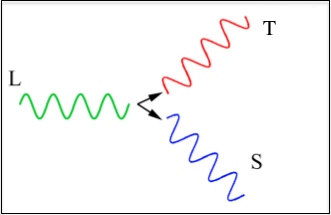
\includegraphics[width=0.5\columnwidth]{Images/Fundamental_emission_Lwaves.png}
\caption[A three wave process of fundamental plasma emission L$\rightarrow$T+S]{A three wave process of fundamental plasma emission L$\rightarrow$T+S. A Langmuir wave decaying into an ion sound wave and an electromagnetic transverse wave at the plasma frequency. (Figure adapted from Solar (interplanetary) Radio Bursts: the Generation of Radio Waves,	an oral presentation by David Malaspina at the Jean Louis Steinberg International Workshop on Solar, Heliospheric and Magnetospheric Radioastronomy, November 2017)}
\label{fig:Femission}
\end{figure}

Second harmonic emission occurs when two Langmuir waves coalesce in the process L+L'$\rightarrow$=T, shown in Figure \ref{fig:Hemission}. Conservation of momentum requires that $\mathbf{k}_L + \mathbf{k'}_L = \mathbf{k}_T$ and for second harmonic (H) generation, $k_T=k_H \approx \frac{\sqrt{3} \omega_p}{c}$. The phase speed $v_\phi$ of Langmuir waves is much less than $\frac{c}{\sqrt{3}}$ meaning that $k_L \gg k_T$ which results in $\mathbf{k}_L \approx -\mathbf{k'}_L$. This means that for a transverse wave at the second harmonic to be created, two Langmuir waves must coalesce almost exactly head on. These backward propagating Langmuir waves are generated: in the three wave processes of L+S$\rightarrow$L' and L$\rightarrow$L'+S; scattering off of thermal ions; and refraction at density inhomogeneities.
 \begin{figure}

     \centering
     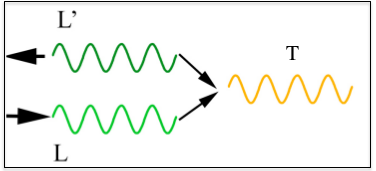
\includegraphics[width=0.5\columnwidth]{Images/Harmonic_emission_Lwaves.png}
     \caption[Three wave process of second harmonic plasma emission L+L' $\rightarrow$ T]{Three wave process of second harmonic plasma emission L+L' $\rightarrow$ T. A Langmuir wave (L) and a backwards propagating Langmuir wave (L') coalesce to form a transverse wave (T) at $2 \omega_p$. (Figure adapted from Solar (interplanetary) Radio Bursts: the Generation of Radio Waves,	an oral presentation by David Malaspina at the Jean Louis Steinberg International Workshop on Solar, Heliospheric and Magnetospheric Radioastronomy, November 2017)}
     \label{fig:Hemission}
 \end{figure}